\documentclass[aspectratio=169]{beamer}
\usetheme{Madrid}
\setbeamertemplate{blocks}[rounded][shadow=false]
% \usecolortheme{beaver}

% Packages
\usepackage[utf8]{inputenc}
\usepackage{graphicx}
\usepackage{booktabs}
\usepackage{amsmath}
\usepackage{amssymb}
\usepackage{tikz}
\usepackage{algorithm}
\usepackage{algpseudocode}
\usepackage{multirow}
\usepackage{adjustbox}

% Theme settings
\setbeamertemplate{footline}{
  \leavevmode%
  \hbox{%
  \begin{beamercolorbox}[wd=.5\paperwidth,ht=2.25ex,dp=1ex,left]{author in head/foot}%
    \usebeamerfont{author in head/foot}\hspace*{2ex}\insertshortauthor
  \end{beamercolorbox}%
  \begin{beamercolorbox}[wd=.5\paperwidth,ht=2.25ex,dp=1ex,right]{date in head/foot}%
    \usebeamerfont{date in head/foot}\insertframenumber{} / \inserttotalframenumber\hspace*{2ex}
  \end{beamercolorbox}}%
  \vskip0pt%
}
% \setbeamertemplate{navigation symbols}{}
% \setbeamertemplate{caption}[numbered]

% Custom colors
% \definecolor{darkblue}{RGB}{0,51,102}
% \definecolor{lightblue}{RGB}{51,153,255}
% \setbeamercolor{structure}{fg=darkblue}
% \setbeamercolor{block title}{bg=darkblue,fg=white}
% \setbeamercolor{block body}{bg=lightblue!10,fg=black}

% Better spacing
\setlength{\leftmargini}{0.8em}
\setlength{\leftmarginii}{0.6em}

% Title information
\title{Method for Optimizing Large Language Models for Edge Devices}
\author{Vinh Pham Xuan}
\institute{
    University of Engineering and Technology, VNU Hanoi\\
    Supervisors: Dr. Vinh Nguyen Van
}
\date{\today}

\begin{document}

% Title slide
\begin{frame}[plain]
    \titlepage
    \begin{center}
        
\includegraphics[height=1.2cm]{figures/uet.jpg}
    \end{center}
\end{frame}


% Problem and Motivation
\begin{frame}[squeeze]{Problem \& Motivation}

\begin{block}{Challenge: Memory \& Compute Demands}
\small
\begin{itemize}
    \item Llama-3.2-3B: \textbf{82.4 GB}, Llama-3.1-8B: \textbf{80+ GB}
    \item Training time: \textbf{3.6h - 9.1h} for 100K samples
\end{itemize}
\end{block}

\vspace{0.1cm}

\begin{block}{Current Limitations}
\small
\begin{itemize}
    \item FP16/BF16 can waste memory
    \item Uniform format assignment
    \item Misses format strengths
\end{itemize}
\end{block}


\end{frame}


% Proposed Approach
\begin{frame}[squeeze]{Proposed Approach: Layer-Wise FP8 Specialization}

\begin{alertblock}{Key Insight}
\small Different transformer components need different precision-range trade-offs
\end{alertblock}

\vspace{0.2cm}

\begin{block}{Strategy: Hybrid Format Assignment}
\small
\begin{itemize}
    \item \textbf{Attention layers}: Use hybrid E4M3 + E5M2
    \begin{itemize}
        \small
        \item Forward pass: \textbf{E4M3} (stable activations)
        \item Backward pass: \textbf{E5M2} (gradient explosions need extended range)
    \end{itemize}
    \item \textbf{MLP layers}: Use only E4M3
    \begin{itemize}
        \small
        \item Both forward \& backward: \textbf{E4M3}
        \item Concentrated distributions $\rightarrow$ Higher precision preferred
    \end{itemize}
\end{itemize}
\end{block}

\vspace{0.2cm}

\begin{alertblock}{Rationale}
\small
\textbf{Attention}: Gradients through softmax have wide dynamic range $\rightarrow$ E5M2 for backward\\
\textbf{MLP}: Feed-forward has narrow range in both directions $\rightarrow$ E4M3 precision
\end{alertblock}

\end{frame}

\begin{frame}[squeeze]{Format Assignment Details}

\begin{columns}[c]
\begin{column}{0.58\textwidth}
    \begin{block}{MLP Components $\rightarrow$ E4M3}
    \small
    \begin{itemize}
        \item Concentrated distributions
        \item Need higher precision, stable computations
    \end{itemize}
    {\footnotesize  \begin{align}
\forall \ell \in \mathcal{L}_{\mathrm{MLP}}: \quad &W_{\ell}, A_{\ell}, G_{\ell} \mapsto \text{E4M3} \label{eq:mlp_assignment}
\end{align}}
    \end{block}


    \begin{block}{Attention $\rightarrow$ E5M2 \& E4M3} 
    \small
    \begin{itemize}
        \item Wide dynamic ranges
        \item Need extended range
    \end{itemize}
    {\footnotesize  \begin{align}
\forall \ell \in \mathcal{L}_{\mathrm{Attn}}: \quad &\begin{cases}
Q_{\ell}, K_{\ell} \mapsto \text{E5M2} \\
V_{\ell}, O_{\ell} \mapsto \text{E4M3} \\
G_{Q,\ell}, G_{K,\ell} \mapsto \text{E5M2} \\
G_{V,\ell}, G_{O,\ell} \mapsto \text{E4M3}
\end{cases} \label{eq:attn_assignment}
\end{align}}
    \end{block}
\end{column}

\begin{column}{0.40\textwidth}
    \centering
    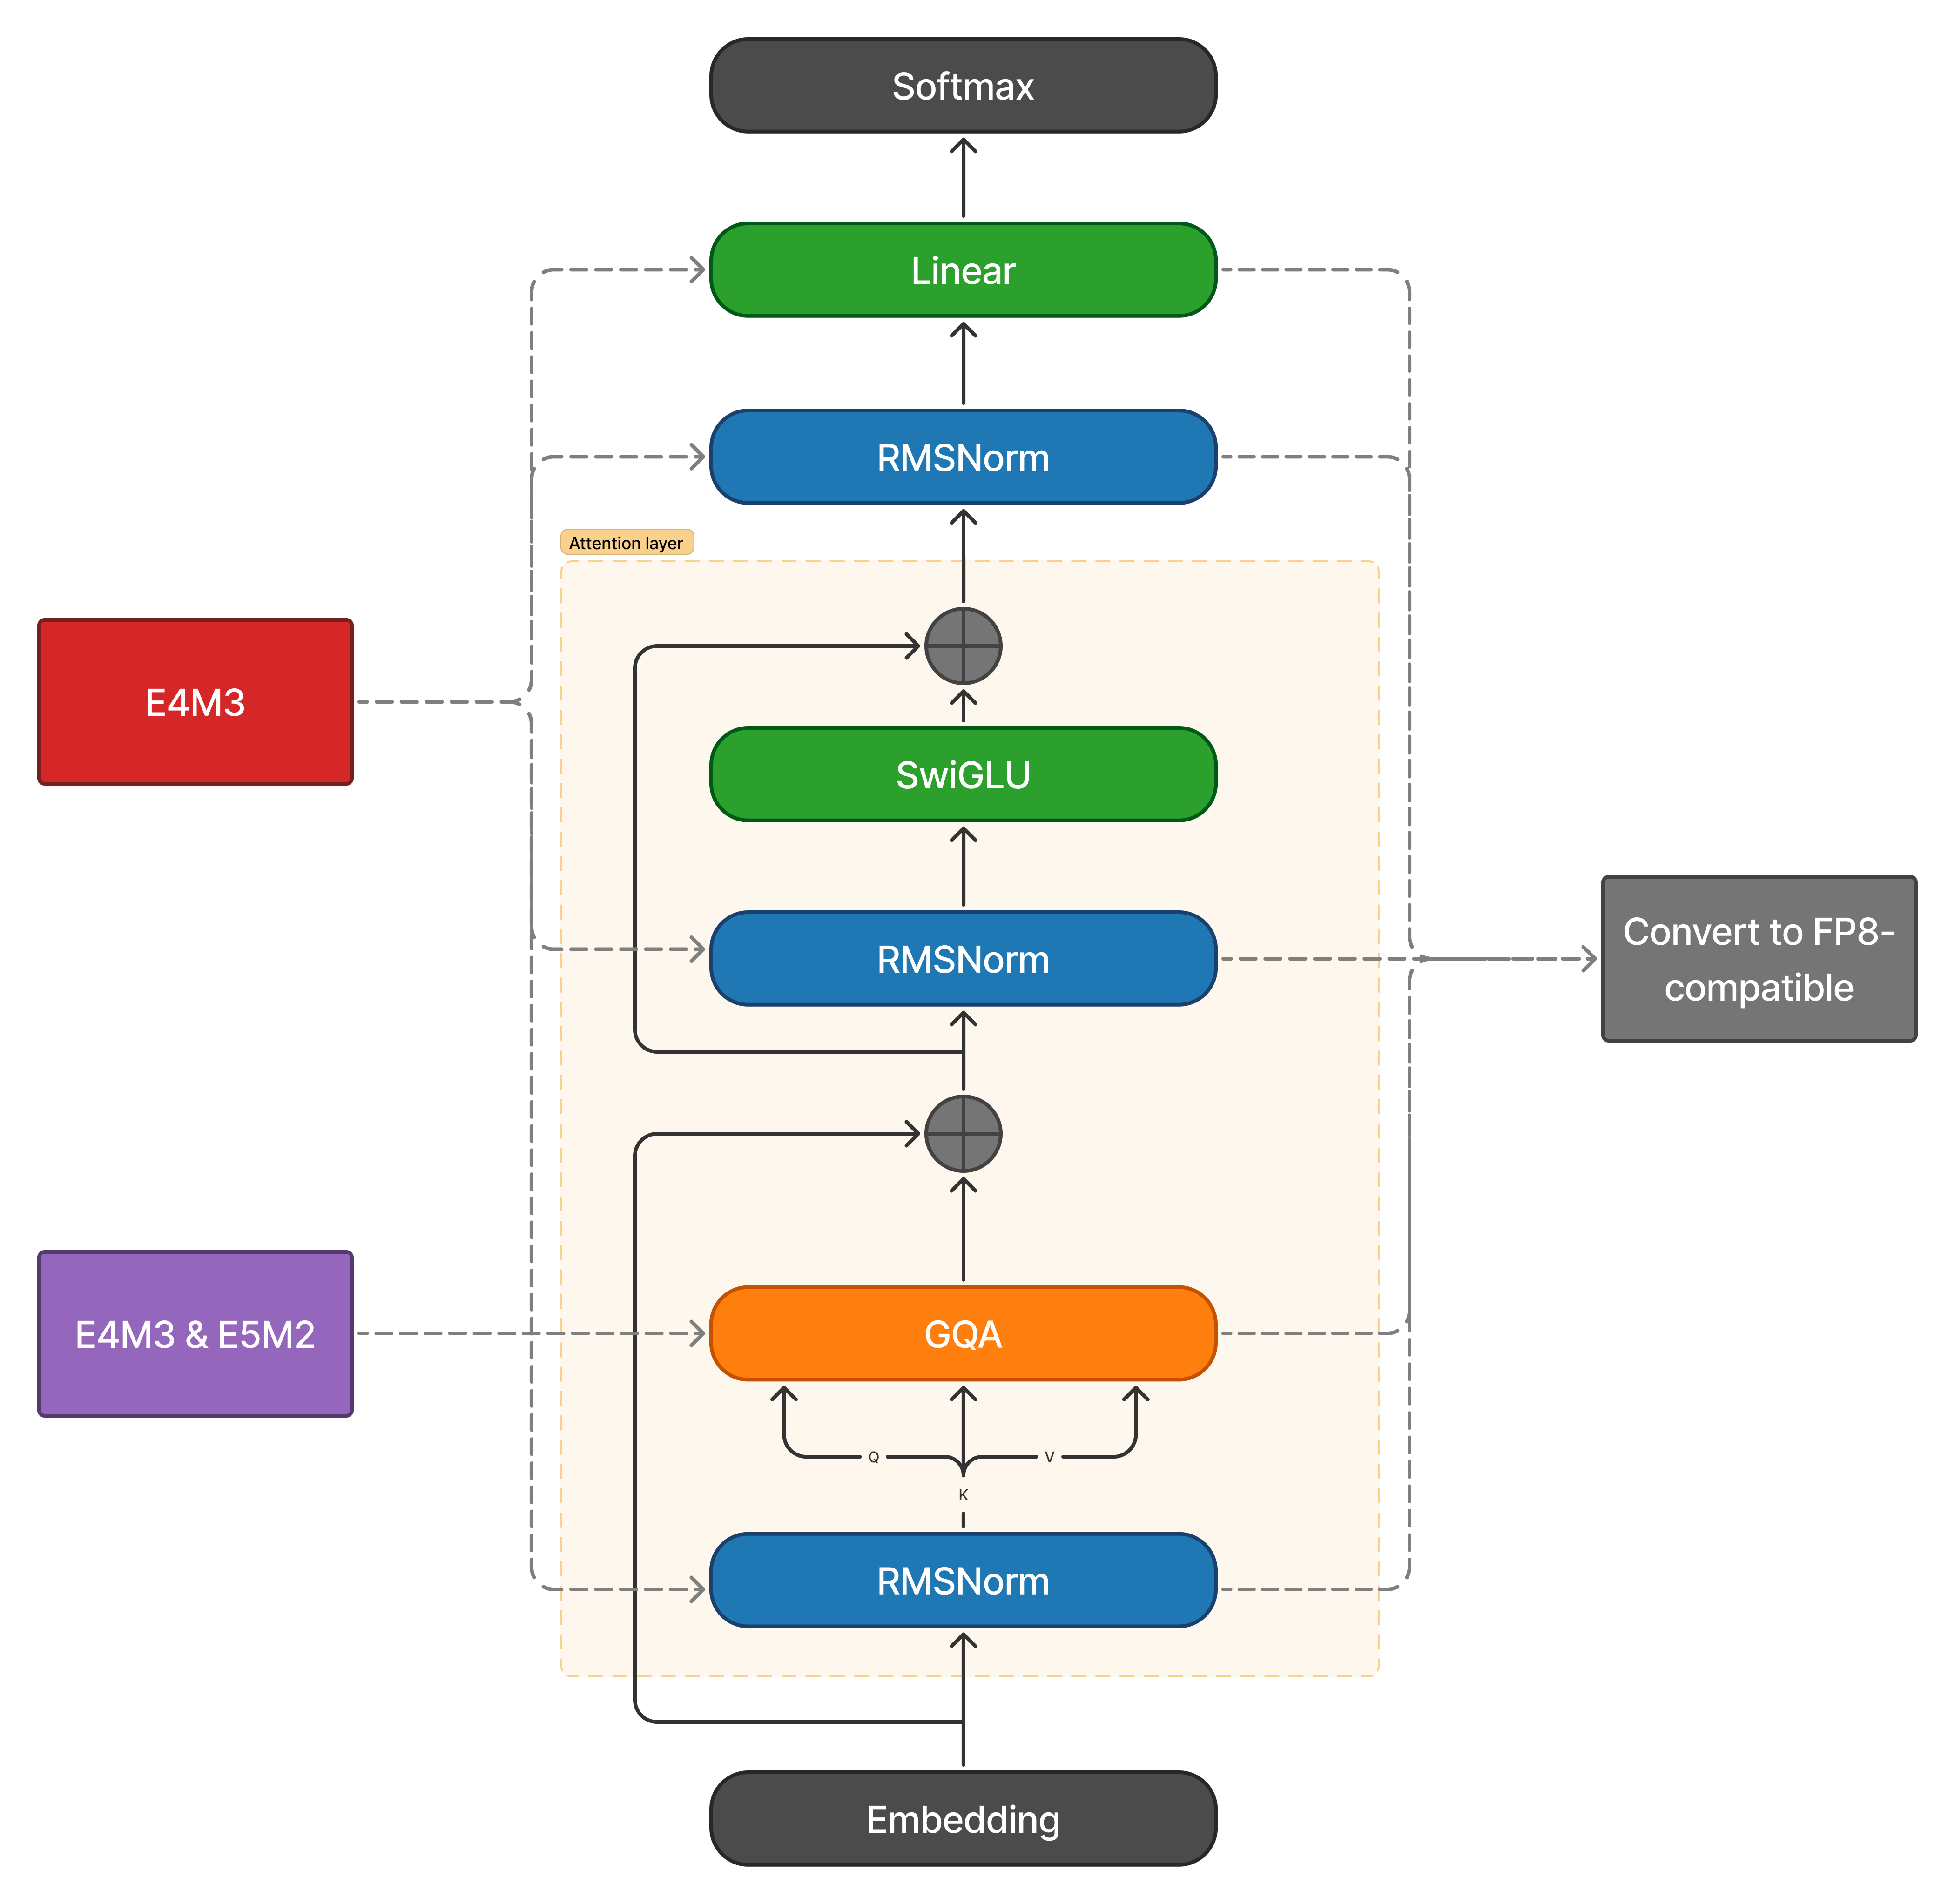
\includegraphics[width=\textwidth]{figures/fp8_convert.png}
    \tiny Layer-wise FP8 assignment
\end{column}
\end{columns}

\end{frame}


% Experimental Setup
\begin{frame}[squeeze]{Experimental Setup}

\begin{columns}[t]
\begin{column}{0.48\textwidth}
    \begin{block}{Models \& Dataset}
    \small
    \begin{itemize}
        \item \textbf{Llama-3.2-3B} \& \textbf{Llama-3.1-8B}
        \item OpenMathInstruct-2 (100K samples)
        \item 3 epochs, seq. length 512
        \item AdamW, lr 1e-5, grad accum. 4
    \end{itemize}
    \end{block}

    \vspace{0.15cm}

    \begin{block}{Hardware}
    \small
    \begin{itemize}
        \item NVIDIA Blackwell GPUs (96 GB)
        \item PyTorch 2.7+, Transformer Engine 2.5.0
    \end{itemize}
    \end{block}
\end{column}

\begin{column}{0.48\textwidth}
    \begin{block}{Baselines Comparison}
    \small
    \begin{enumerate}
        \item \textbf{BF16} {\footnotesize (mixed precision)}

        \item \textbf{Hybrid FP8} {\footnotesize (delayed scaling)}

        \item \textbf{Ours} {\footnotesize (layer-wise FP8)}
    \end{enumerate}
    \end{block}
\end{column}
\end{columns}

\vspace{0.2cm}

\begin{alertblock}{Evaluation Metrics}
\small
Training time • Memory usage • Loss variance • Perplexity • Convergence
\end{alertblock}

\end{frame}


% Results - Performance
\begin{frame}[squeeze]{Results: Performance Improvements}

\begin{columns}[c]
\begin{column}{0.55\textwidth}
    \begin{block}{Training Time Reduction}
    \small
    \begin{tabular}{@{}lcc@{}}
    \toprule
    \textbf{Model} & \textbf{BF16} & \textbf{Ours} \\
    \midrule
    3B & 3.6 h & \textbf{2.1 h} \\
    & & {\footnotesize \textcolor{blue}{42\% faster}} \\
    \midrule
    8B & 9.1 h & \textbf{6.6 h} \\
    & & {\footnotesize \textcolor{blue}{27\% faster}} \\
    \bottomrule
    \end{tabular}
    \end{block}

    \vspace{0.15cm}

    \begin{block}{Memory Efficiency (3B)}
    \small
    82.4 GB $\rightarrow$ \textbf{74.2 GB} (\textcolor{blue}{10\% $\downarrow$})
    \end{block}

    \vspace{0.15cm}

    \begin{alertblock}{Key Findings}
    \small
    1.3-1.7$\times$ speedup • Scales favorably • Beats Hybrid
    \end{alertblock}
\end{column}

\begin{column}{0.42\textwidth}
    \centering
    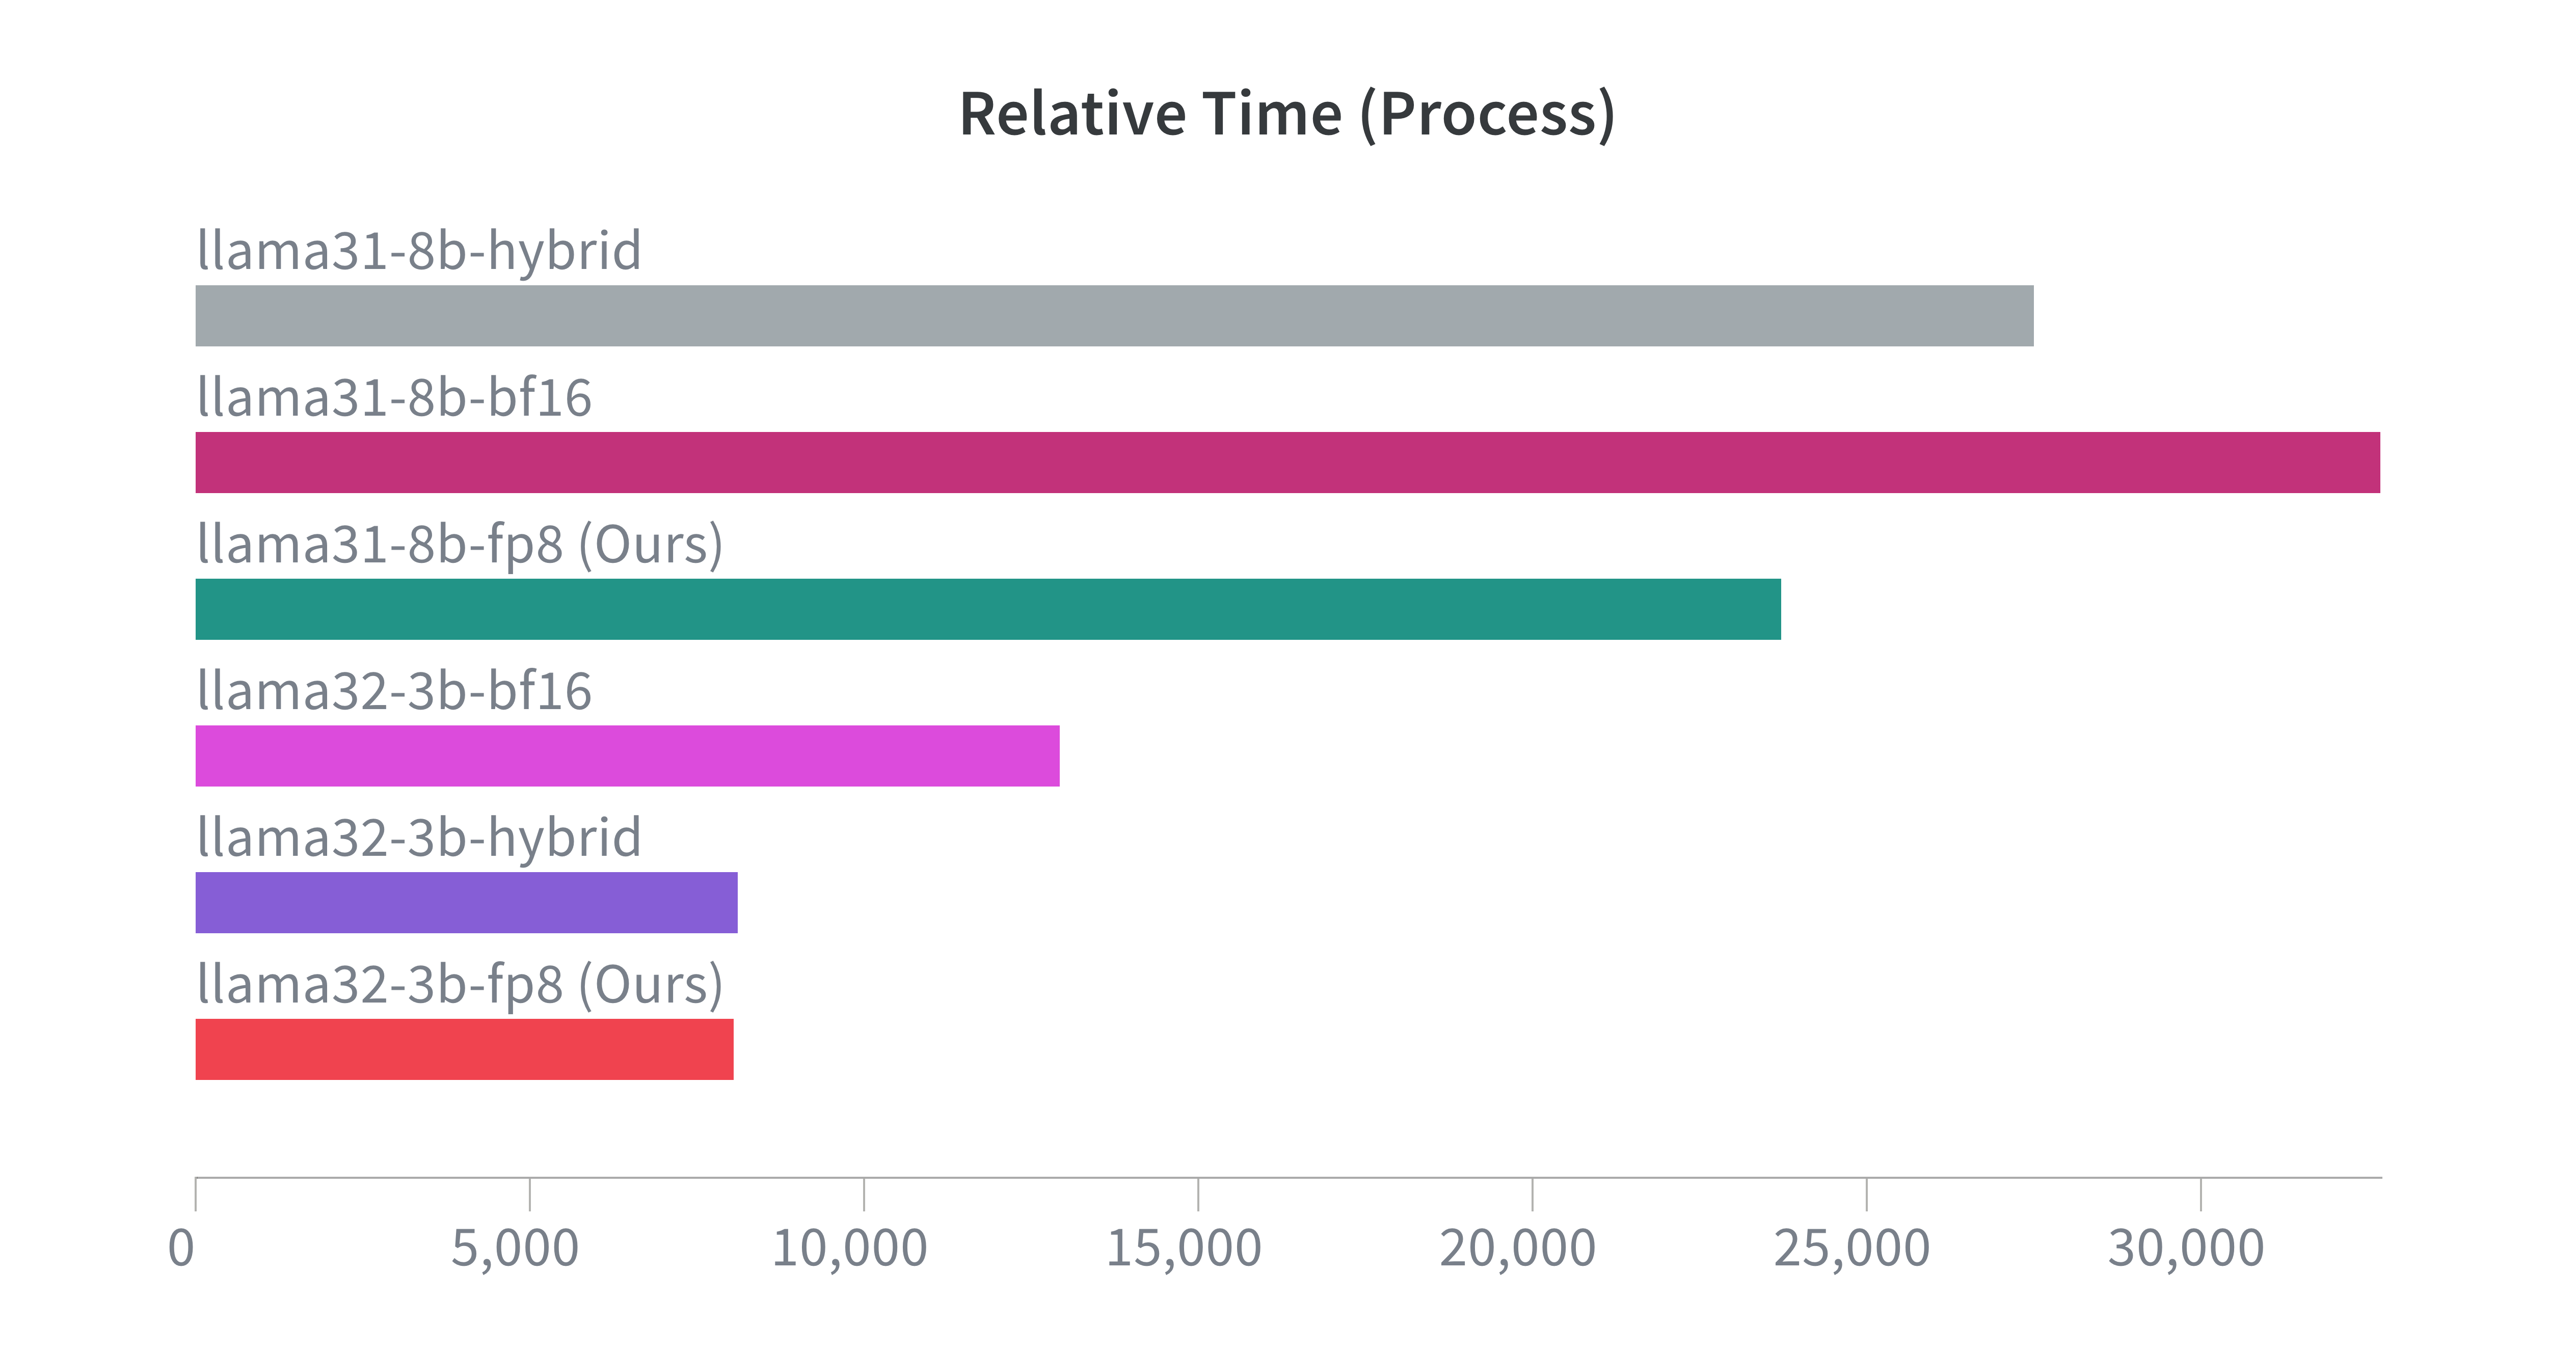
\includegraphics[width=\textwidth]{figures/training_time.png}
    {\tiny Training time comparison}
\end{column}
\end{columns}

\end{frame}


% Results - Stability (Loss Variance)
\begin{frame}{Results: Loss Variance Analysis}

\begin{columns}[c]
\begin{column}{0.4\textwidth}
    \begin{block}{Loss Variance Comparison}
    
    \vspace{0.2cm}
    \begin{itemize}
        \item Our method: \textbf{$<$ 0.4}
        \item Hybrid FP8: Spikes \textbf{$\geq$ 0.8}
        \item \textcolor{blue}{\textbf{50\% lower variance}}
    \end{itemize}
    \end{block}

    \vspace{0.3cm}

    \begin{alertblock}{Why More Stable?}
    \begin{itemize}
        \item E5M2 for Q/K paths
        \item Prevents overflow/underflow
        \item E4M3 for MLP stability
        \item Component-aware design
    \end{itemize}
    \end{alertblock}
\end{column}

\begin{column}{0.60\textwidth}
    \centering
    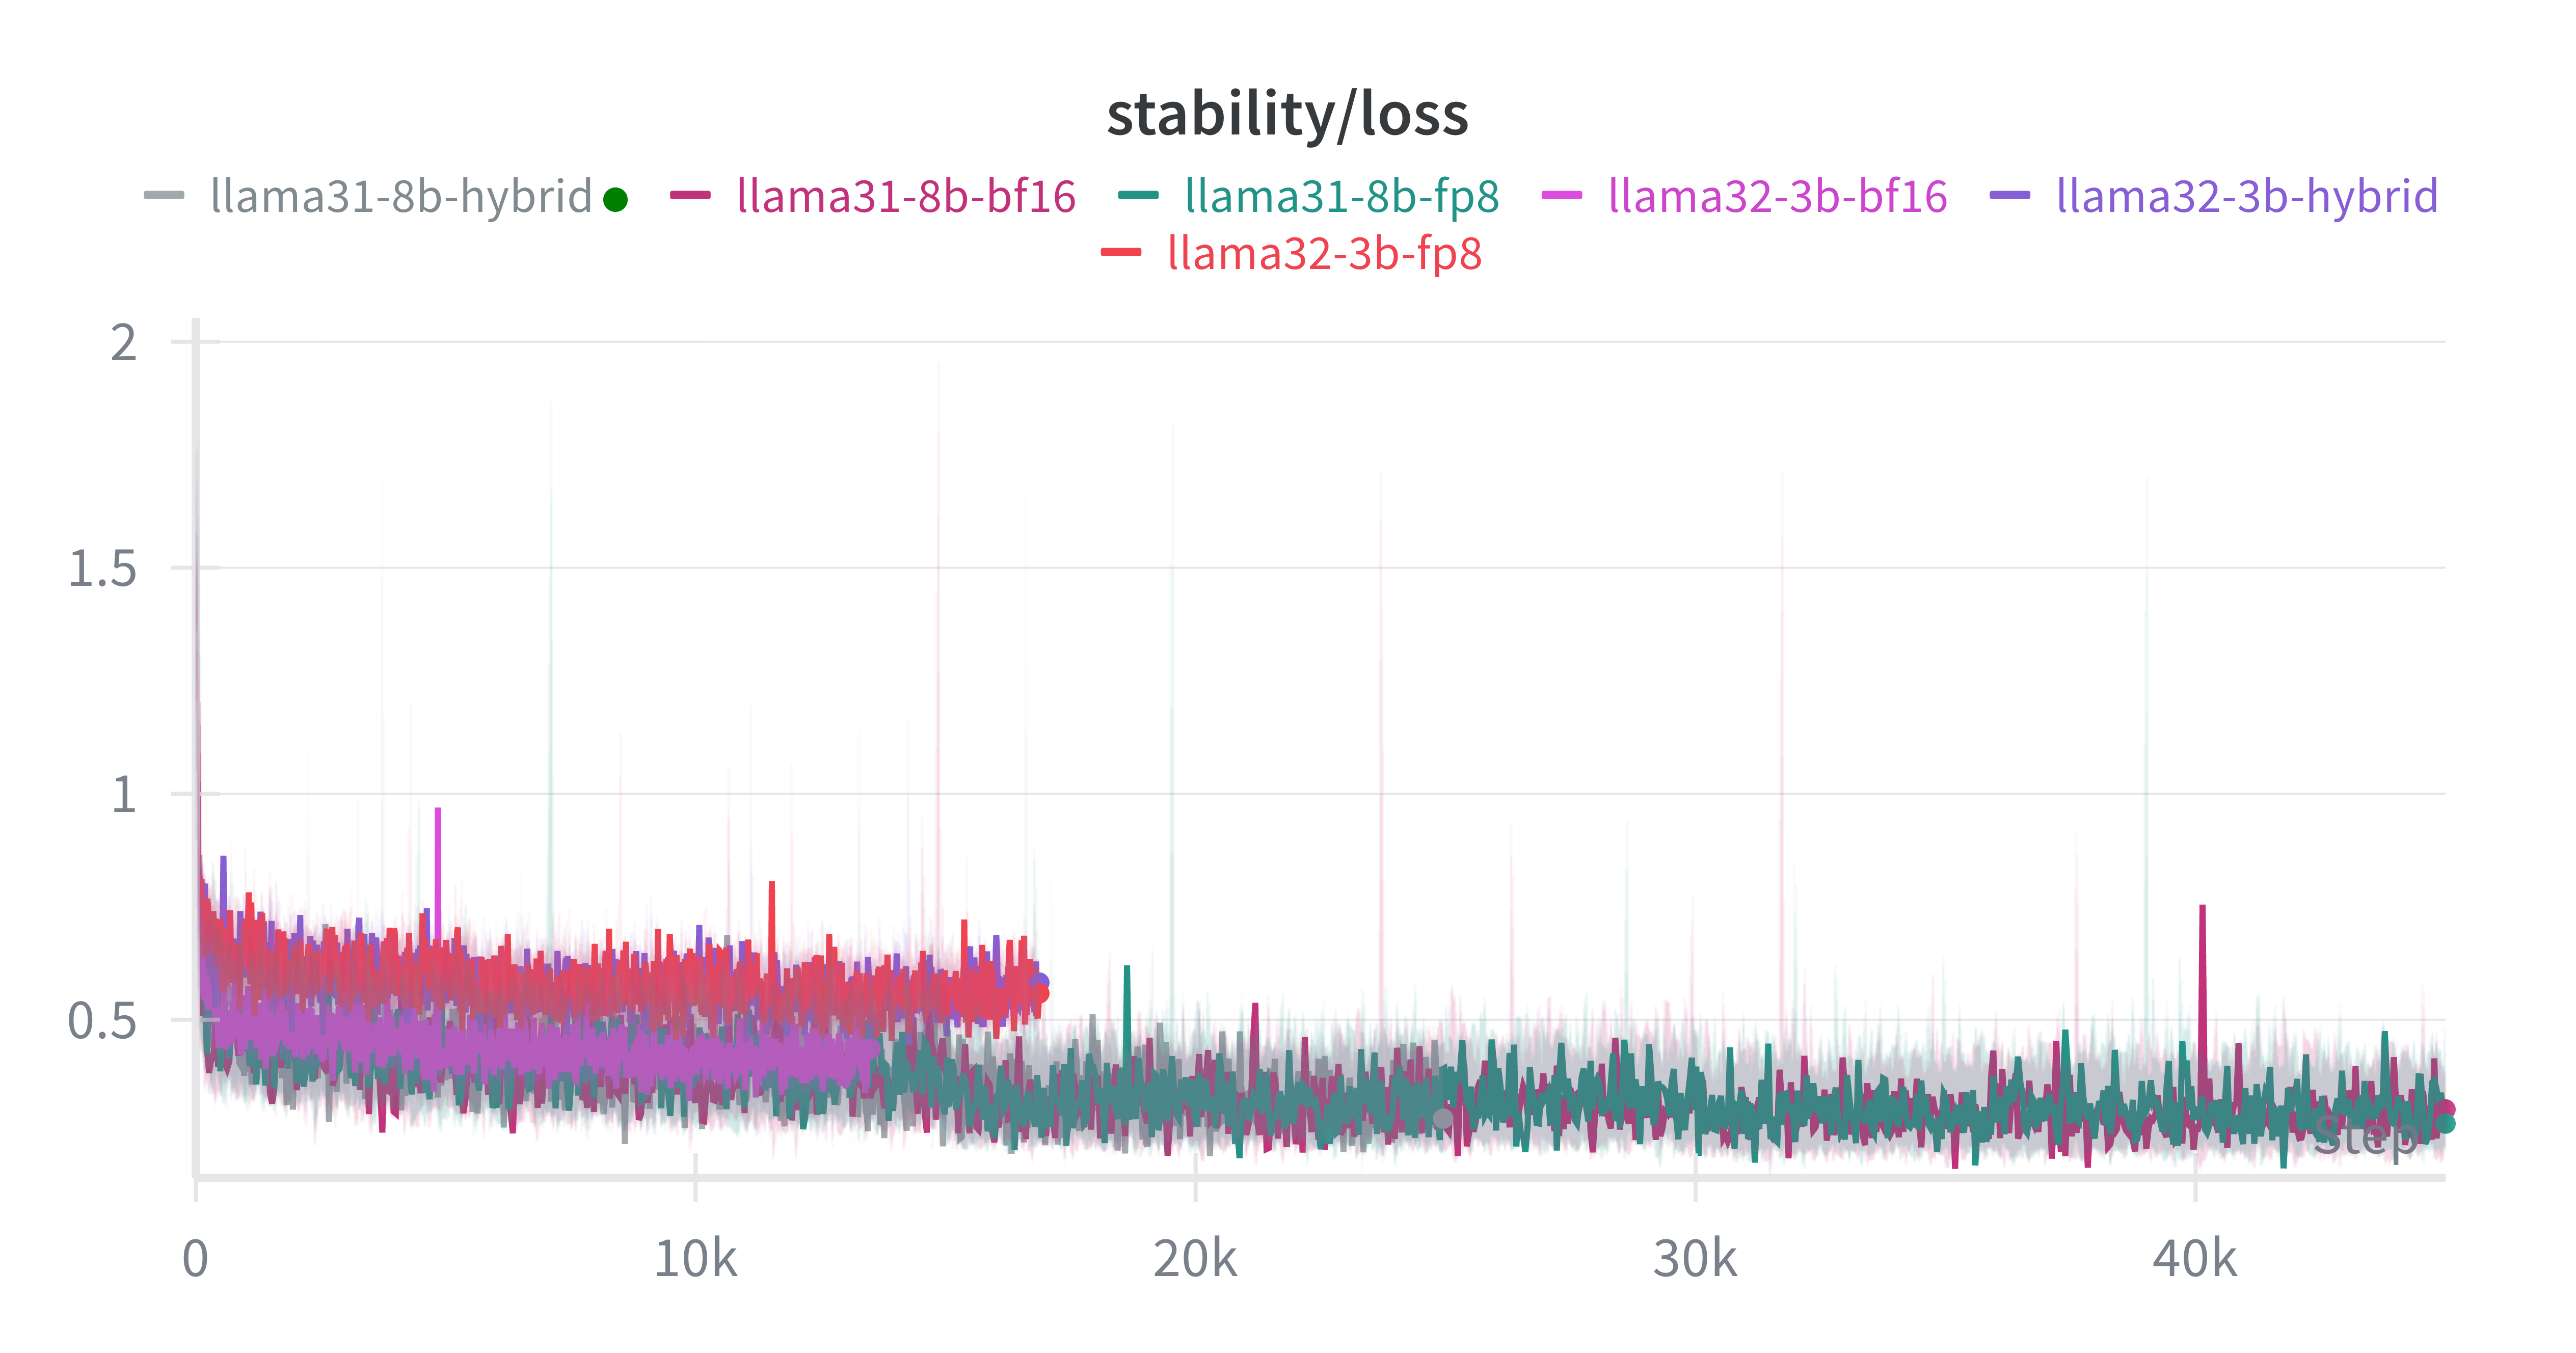
\includegraphics[width=\textwidth]{figures/numeric_stability.png}

    \vspace{0.3cm}

    \small
    \textbf{Key Observation:} Layer-wise FP8 maintains consistent low variance throughout training, while Hybrid FP8 shows periodic instability spikes.
\end{column}
\end{columns}
\vspace{0.3cm}
\tiny
    Variance: $\sigma^2 = \frac{1}{n}\sum_{i=1}^{n}(L_i - \bar{L})^2$

\end{frame}


% Results - Convergence Quality
\begin{frame}{Results: Convergence Quality}

\begin{columns}[c]
\begin{column}{0.48\textwidth}
    \begin{block}{Training Convergence}
    \begin{itemize}
        \item Initial loss: \textbf{0.47}
        \item Final loss: \textbf{0.36}
        \item Perplexity: \textbf{1.30-1.32}
        \item Comparable to BF16
    \end{itemize}
    \end{block}

    \vspace{0.3cm}

    \begin{block}{Convergence Characteristics}
    \begin{itemize}
        \item Smooth loss curve
        \item No divergence issues
        \item Stable throughout training
        \item Maintained model quality
    \end{itemize}
    \end{block}
\end{column}

\begin{column}{0.50\textwidth}
    \centering
    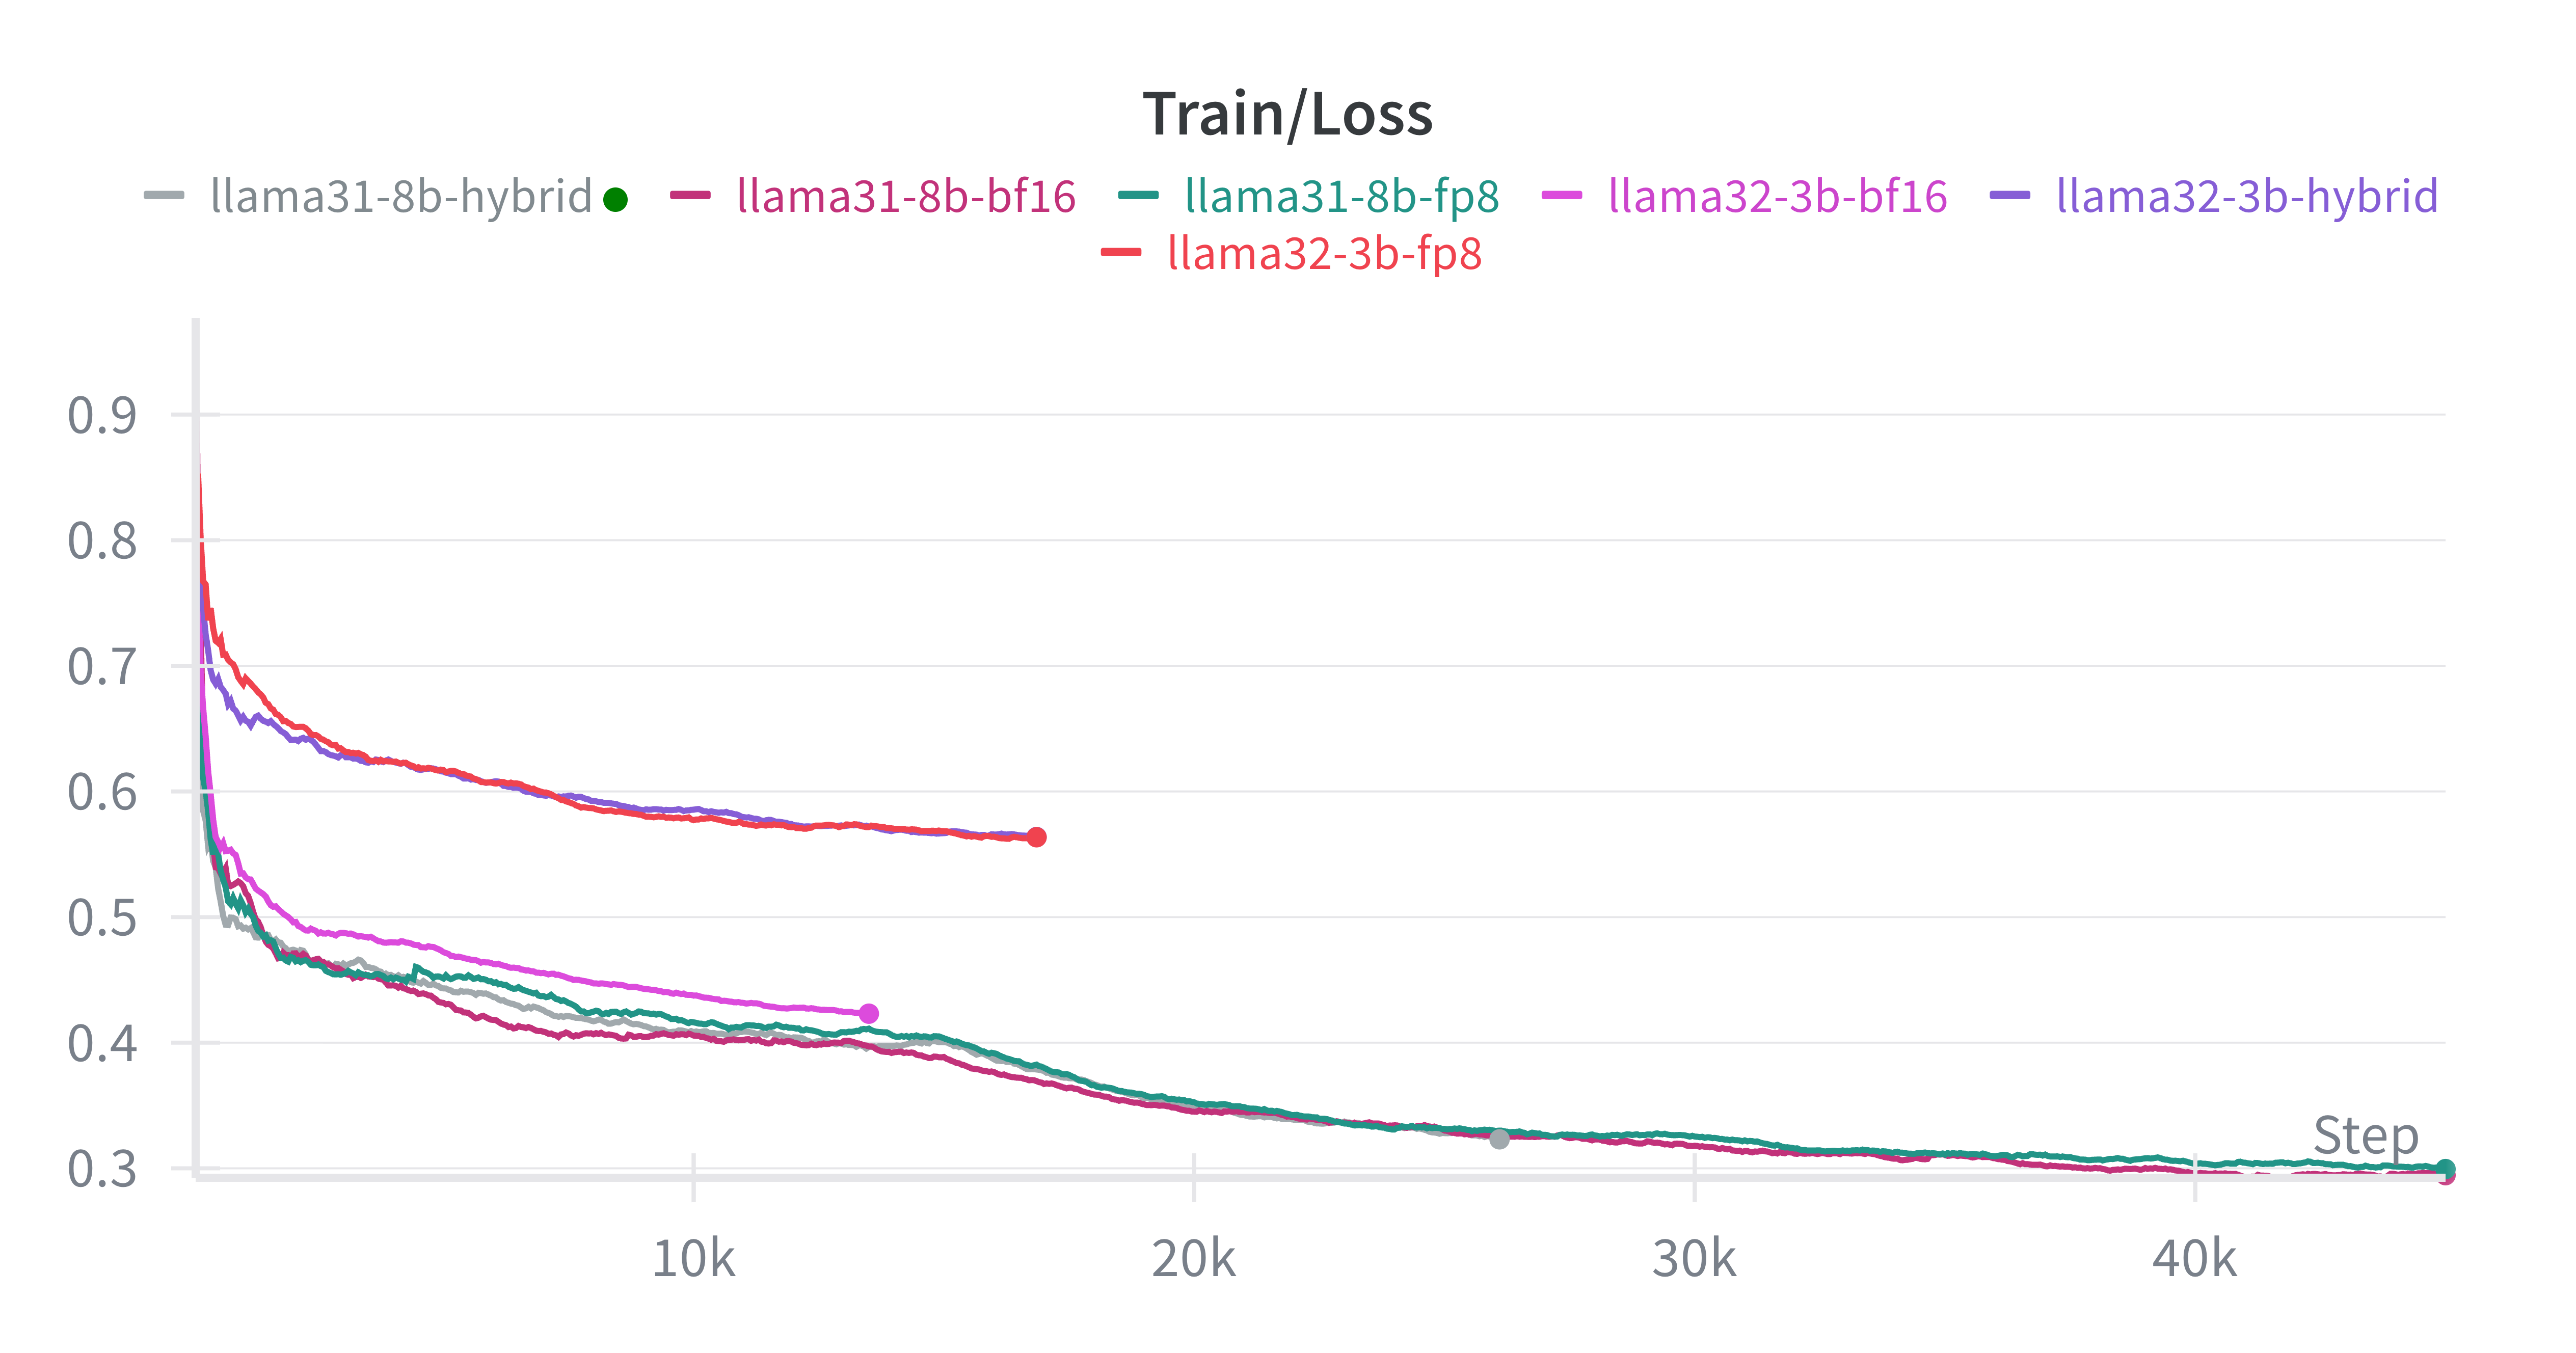
\includegraphics[width=\textwidth]{figures/avg_loss.png}

    \vspace{0.3cm}

    \small
    \textbf{Key Finding:} Layer-wise FP8 achieves comparable final loss and perplexity to BF16 baseline with smoother training dynamics.
\end{column}
\end{columns}

\end{frame}


% Results - Training Perplexity
\begin{frame}{Results: Training Perplexity}

\begin{columns}[c]
\begin{column}{0.48\textwidth}
    \begin{block}{Perplexity Comparison}
    \small
    \begin{itemize}
        \item Layer-wise FP8 matches BF16 baseline
        \item Hybrid FP8 shows higher perplexity
        \item Consistent convergence behavior
    \end{itemize}
    \end{block}

    \vspace{0.3cm}

    \begin{alertblock}{Key Insight}
    \small
    Component-aware format assignment preserves model quality while achieving significant speedup
    \end{alertblock}
\end{column}

\begin{column}{0.50\textwidth}
    \centering
    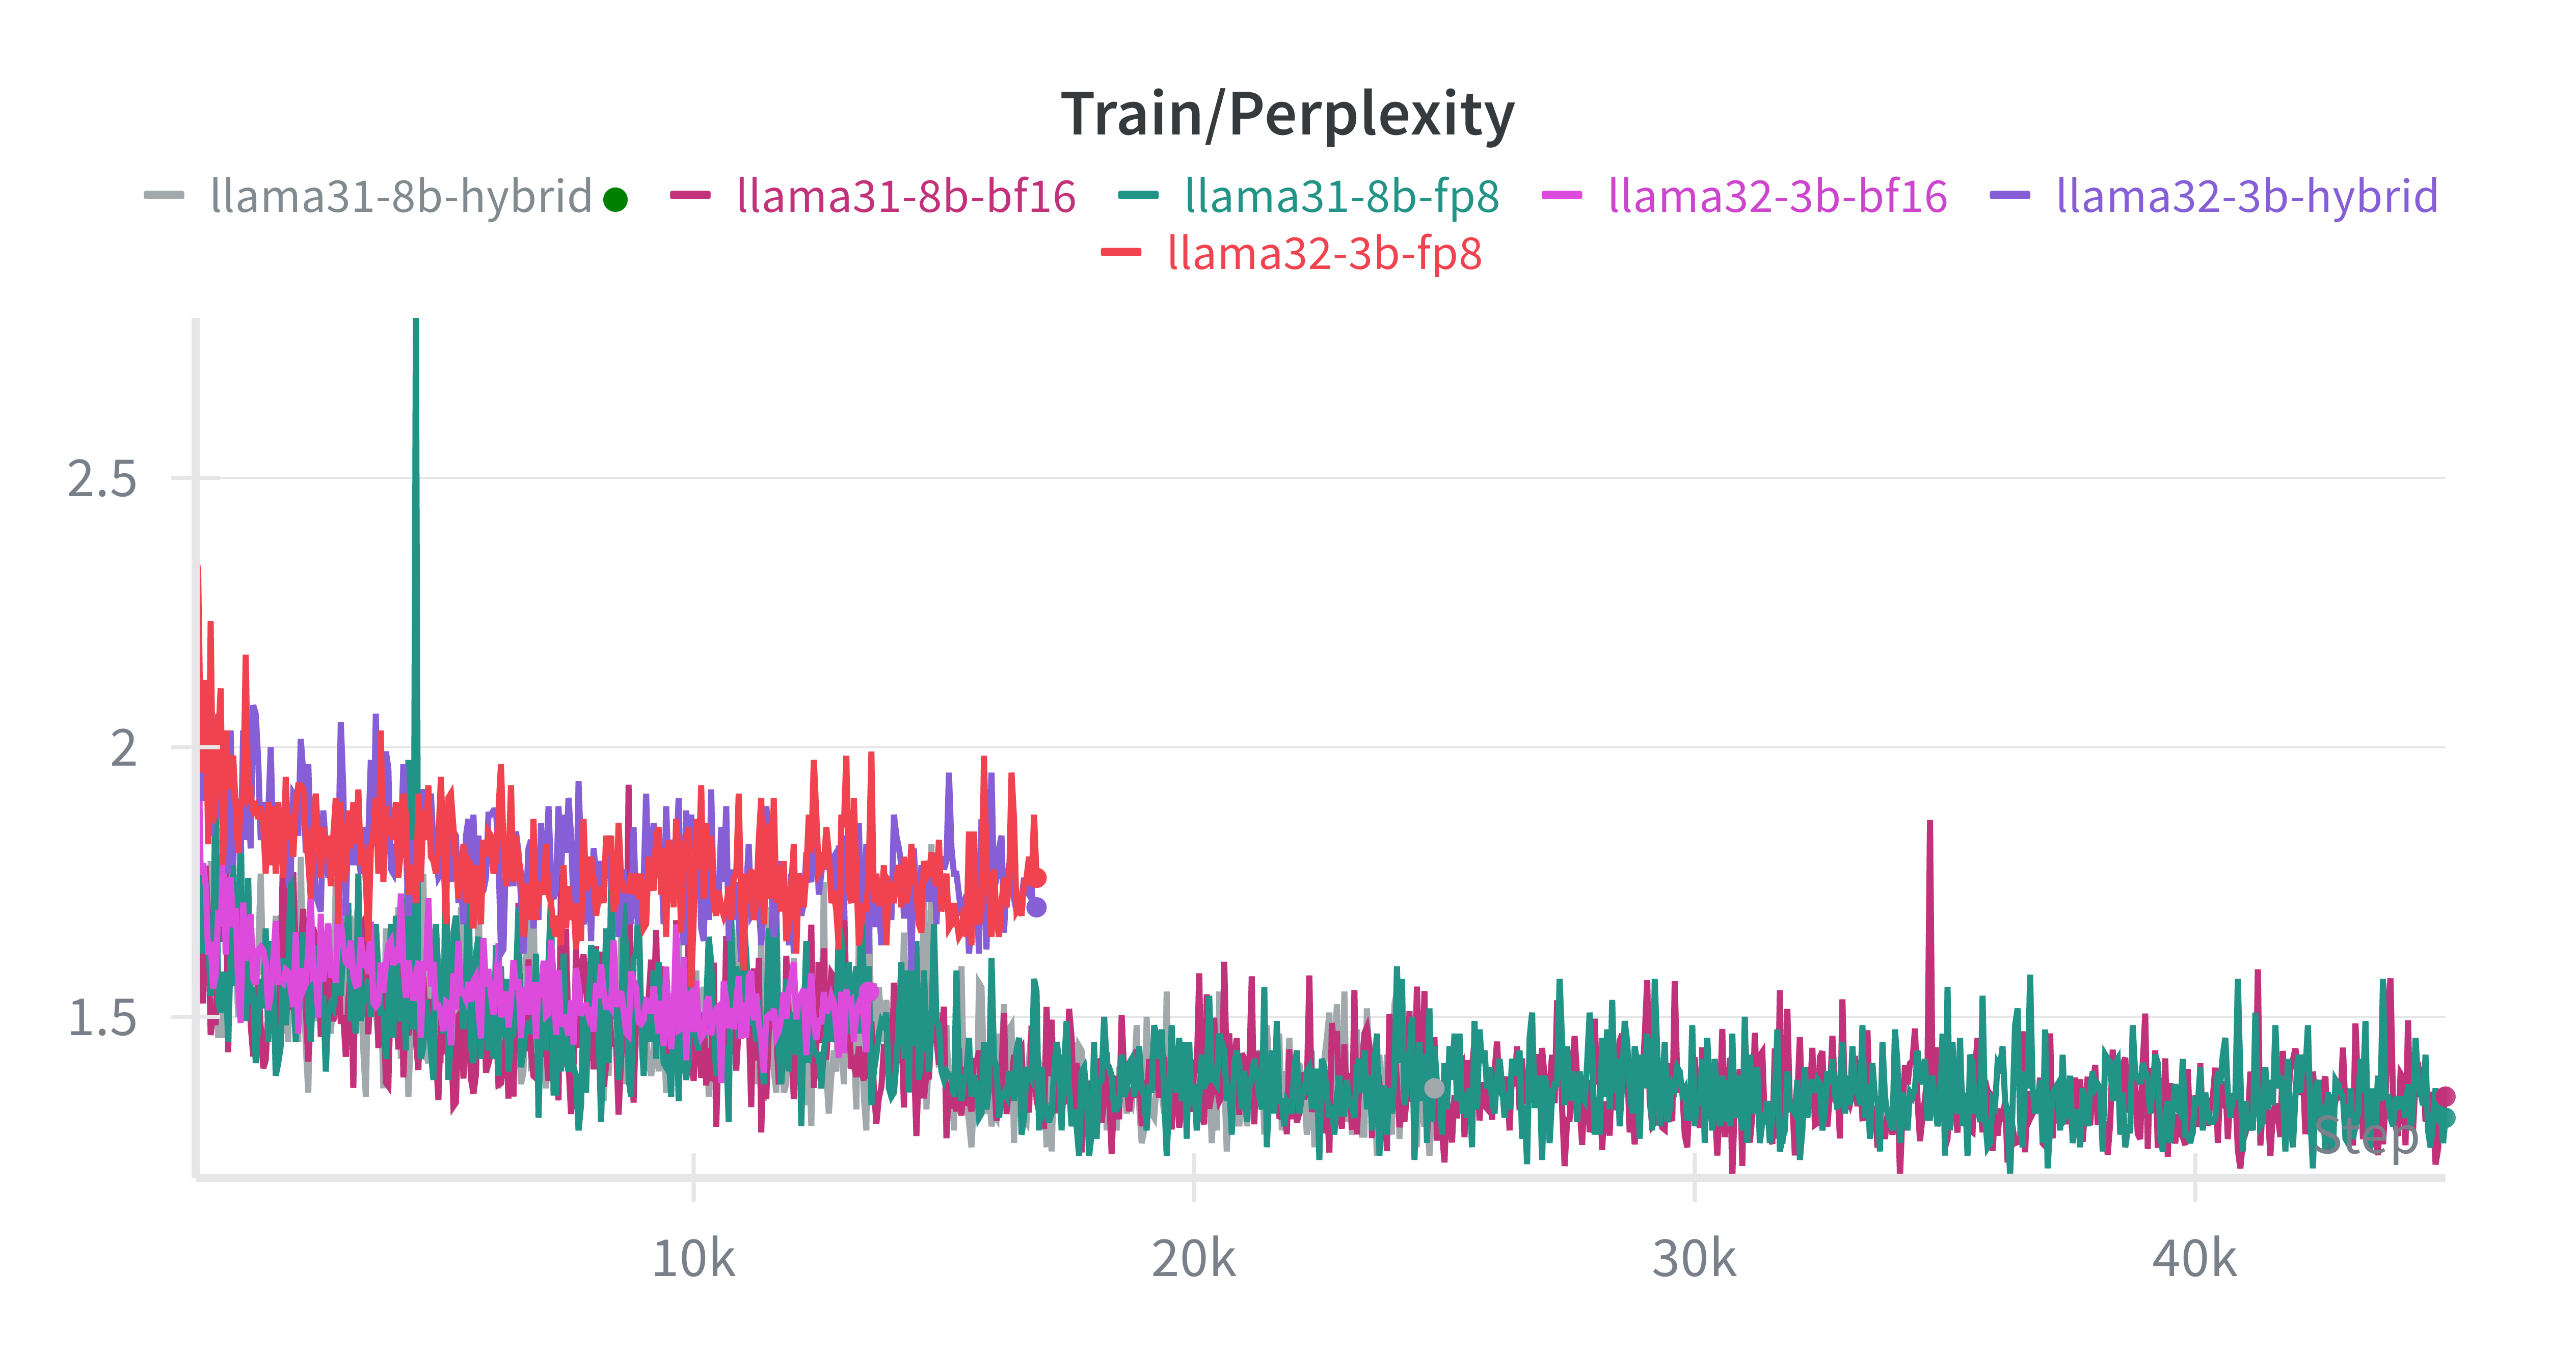
\includegraphics[width=\textwidth]{figures/train_perplexity.png}

    \vspace{0.3cm}

    \small
    \textbf{Observation:} Layer-wise FP8 maintains perplexity close to BF16, demonstrating effective precision-range trade-off.
\end{column}
\end{columns}

\end{frame}


% Conclusion and Future Work
\begin{frame}{Conclusion \& Future Work}

\begin{alertblock}{Summary of Achievements}
\small
\textbf{3B:} 10\% memory $\downarrow$, 42\% time $\downarrow$ \quad \textbf{8B:} 27\% time $\downarrow$ \quad \textbf{50\% lower variance}
\end{alertblock}

\vspace{0.2cm}

\begin{columns}[t]
\begin{column}{0.32\textwidth}
    \begin{block}{Key Results}
    \small
    \begin{itemize}
        \item Layer-wise FP8 works!
        \item Scales favorably
        \item Superior stability
        \item Maintained quality
    \end{itemize}
    \end{block}
\end{column}

\begin{column}{0.32\textwidth}
    \begin{block}{Limitations}
    \small
    \begin{itemize}
        \item Blackwell/Hopper
        \item 3B \& 8B only
        \item Memory @ 8B
        \item Math reasoning
    \end{itemize}
    \end{block}
\end{column}

\begin{column}{0.32\textwidth}
    \begin{block}{Future Work}
    \small
    \begin{itemize}
        \item 70B+ models
        \item Dynamic formats
        \item Memory optim.
        \item More tasks
    \end{itemize}
    \end{block}
\end{column}
\end{columns}

\vspace{0.5cm}

\begin{center}
\Large \textbf{Thank You!}\\
\vspace{0.3cm}
\normalsize \textit{Questions?}
\end{center}

\end{frame}


\end{document}
